\documentclass[11pt,a4paper]{article}
\usepackage[a4paper,margin=1in]{geometry}
\usepackage{graphicx}
\usepackage{xcolor}
\usepackage{longtable}
\usepackage{booktabs}
\usepackage{url}
\usepackage{caption}
\usepackage{array}
\definecolor{osdaggreen}{HTML}{91B014}
\title{\textbf{OsdagBridge LaTeX Report Generator}\\[2mm]
\large Refactoring \& Enhancements --- Technical Report}
\author{FOSSEE Winter Internship Screening Task}
\date{November 2026}
\begin{document}
\maketitle

\section{Overview}
The report generator assembles a multi-chapter LaTeX document from Python modules under
\path{src/osdagbridge/core/reports/}. The original implementation scattered formatting constants across the preamble and chapters, lost table headers at page breaks, allowed content to approach the footer, merged vehicle and footway loads, and contained no data visualisation. All six requested improvements were implemented and verified against a real OpenSees analysis.

\section{Requirement status}
\begin{longtable}{p{0.32\linewidth}p{0.60\linewidth}}
\toprule
\textbf{Requirement} & \textbf{Implementation and evidence} \\
\midrule
Repeating table headers &
Central post-processor inserts \textbackslash endfirsthead / \textbackslash endhead into every longtable.
Count: \textbf{2 (before) $\rightarrow$ 50 (after)}. Verified on Table 5.22 continuation pages. \\
Layout / footer / spacing &
Central 8-line page-bottom threshold, \textbackslash needspace before tables and headings, central table padding/rules, fixed ``Page X of ??'' footer. \\
Load table refactoring &
Separate \emph{Vehicle Live Loads} and \emph{Footway Live Load} tables; rows driven by the \texttt{KEY\_LL\_*} selections. Braking 217.39\,kN; centrifugal 91.29\,kN (IRC 6 Cl.\,209). \\
Utilization Ratio chart &
Section 5.5 bar chart for girder, deck, cross bracing and end diaphragm; red dashed UR=1.0 line; pass/fail colours. \\
Material quantity charts &
Chapter 7 three-panel chart: steel tonnage, concrete volume, rebar weight. Charts saved as temporary PNGs and embedded via a shared figure helper. \\
Centralized styles &
New \path{styles.py} owns geometry, palette, padding, header/footer theme, Matplotlib rcParams and the global LaTeX pass. Every chapter now imports it. \\
\bottomrule
\end{longtable}

\section{Files changed}
\begin{itemize}
\item \path{src/osdagbridge/core/reports/styles.py} (new) --- single source of truth.
\item \path{src/osdagbridge/core/reports/charts.py} (new) --- Matplotlib chart generation.
\item \path{report\_generator.py}, \path{chap1.py}--\path{chap9.py}, \path{executive\_summary.py} --- consume styles; new charts in Chapters 3, 5, 7.
\item \path{src/osdagbridge/core/utils/common.py} --- new centrifugal-load keys.
\item \path{src/osdagbridge/core/utils/codes/irc6\_2017.py} --- fixed braking-force helper.
\item \path{scripts/generate\_sample\_reports.py}, \path{scripts/gui\_smoke\_test.py}, \path{scripts/run\_full\_design\_test.py} (new).
\item \path{scripts/tex/lastpage.sty}, \path{scripts/tex/makecell.sty} (new) --- minimal TeX compatibility stubs.
\item \path{tests/unit/test\_report\_styles.py} (new) --- 3 regression tests.
\end{itemize}

\section{Centralized style architecture}
\path{styles.py} exposes: document settings (\texttt{PAGE\_MARGIN}, \texttt{DOCUMENT\_STRETCH}); colour palette (\texttt{COLOR\_OSDAG\_GREEN\_HEX}, \texttt{COLOR\_UR\_PASS}, \texttt{COLOR\_UR\_FAIL}); table layout (\texttt{TAB\_COLSEP}, \texttt{ARRAY\_STRETCH}, \texttt{PAGE\_BOTTOM\_THRESHOLD\_LINES}, \texttt{table\_header\_row()}); spacing constants (\texttt{SECTION\_SKIP}, \texttt{TABLE\_TOP\_SKIP}, \texttt{FIGURE\_SKIP}); chart theming (\texttt{matplotlib\_rc()}, \texttt{figure\_block()}); and the global pass \texttt{apply\_global\_styles()} which repeats longtable headers and protects headings from the footer.

\section{Verification performed}
\begin{longtable}{p{0.30\linewidth}p{0.62\linewidth}}
\toprule
\textbf{Test} & \textbf{Result} \\
\midrule
Unit tests & 3 passed (styles post-processor). \\
Sample PDF build & \path{Report\_Before.pdf} 42 pages; \path{Report\_After.pdf} 43 pages; no LaTeX errors. \\
GUI report path & Real dialog $\rightarrow$ QThread worker $\rightarrow$ \texttt{generate\_design\_report}; \path{Report\_From\_GUI.pdf} produced. \\
Real solver run & Real OpenSees analysis + IRC 22 design, 4 girders / 30\,m, 997 output keys; \path{Report\_Real\_Design.pdf} (53 pages). \\
Page 30 / G4 & G4 rows end well clear of the footer; continued header repeated. \\
\bottomrule
\end{longtable}

\section{Visual evidence}
\begin{figure}[htbp]
\centering
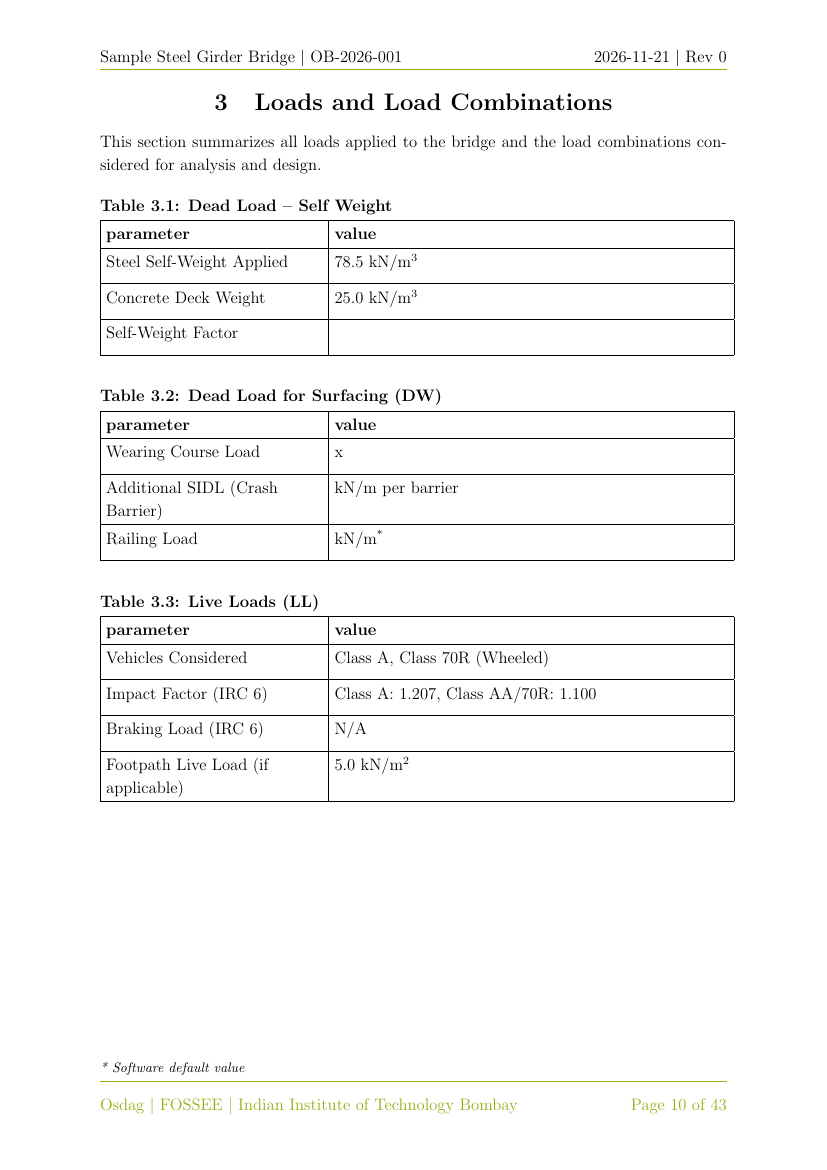
\includegraphics[width=0.78\linewidth]{report_assets/before_loads}
\caption{Baseline: merged Live Loads table.}
\end{figure}
\begin{figure}[htbp]
\centering
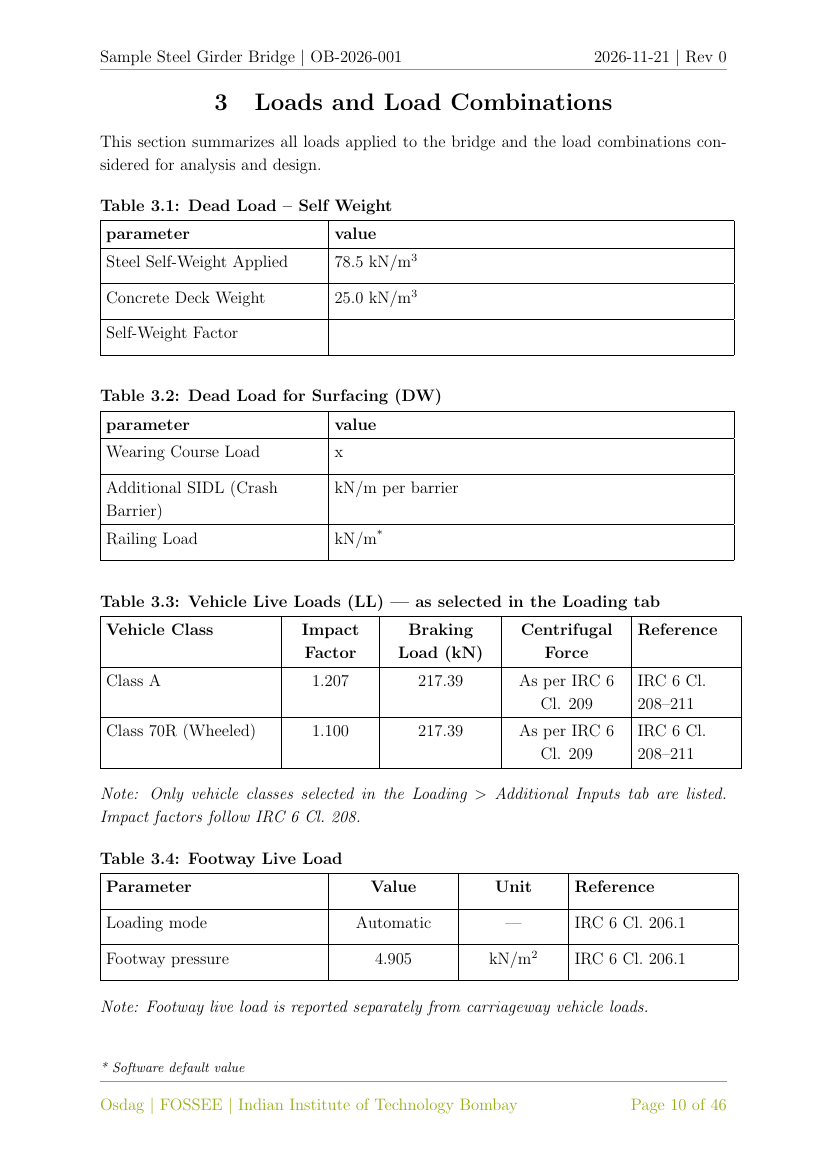
\includegraphics[width=0.78\linewidth]{report_assets/after_loads}
\caption{Enhanced: separate vehicle and footway tables with unit columns.}
\end{figure}
\begin{figure}[htbp]
\centering
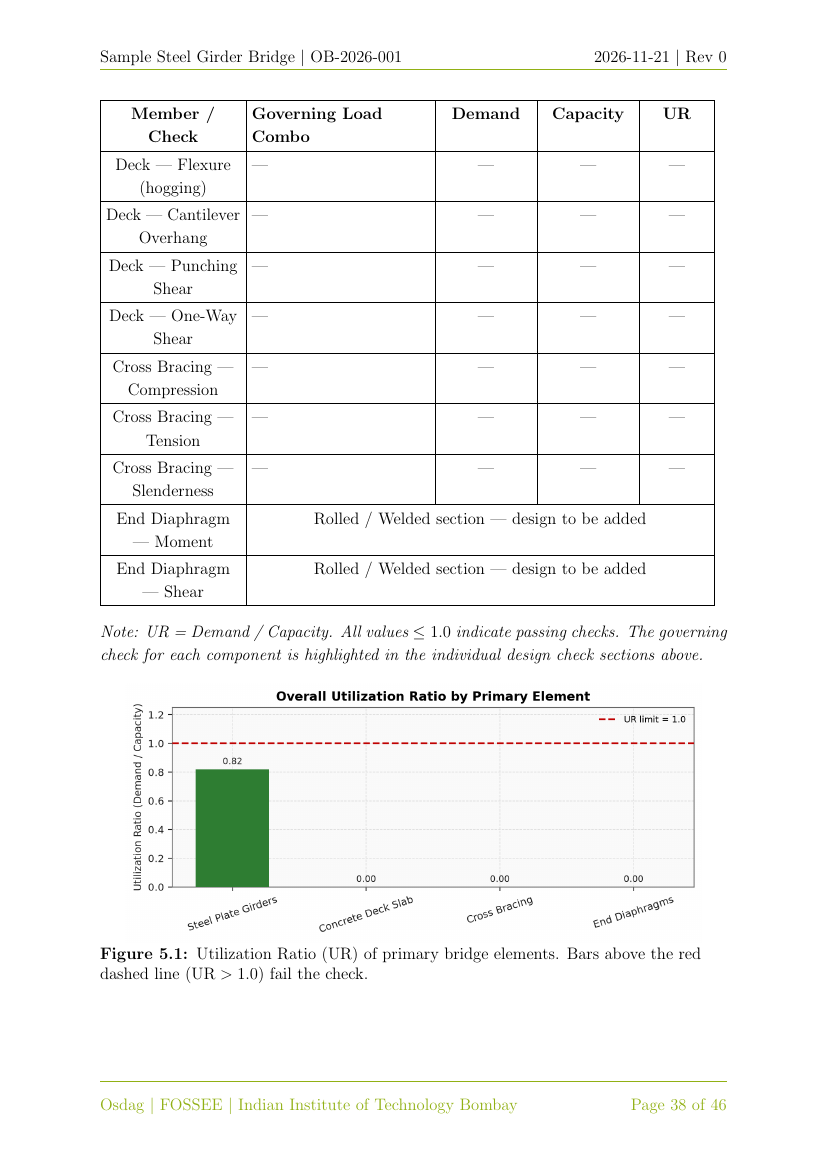
\includegraphics[width=0.78\linewidth]{report_assets/ur_chart}
\caption{Utilization Ratio chart with UR=1.0 threshold (Section 5.5).}
\end{figure}
\begin{figure}[htbp]
\centering
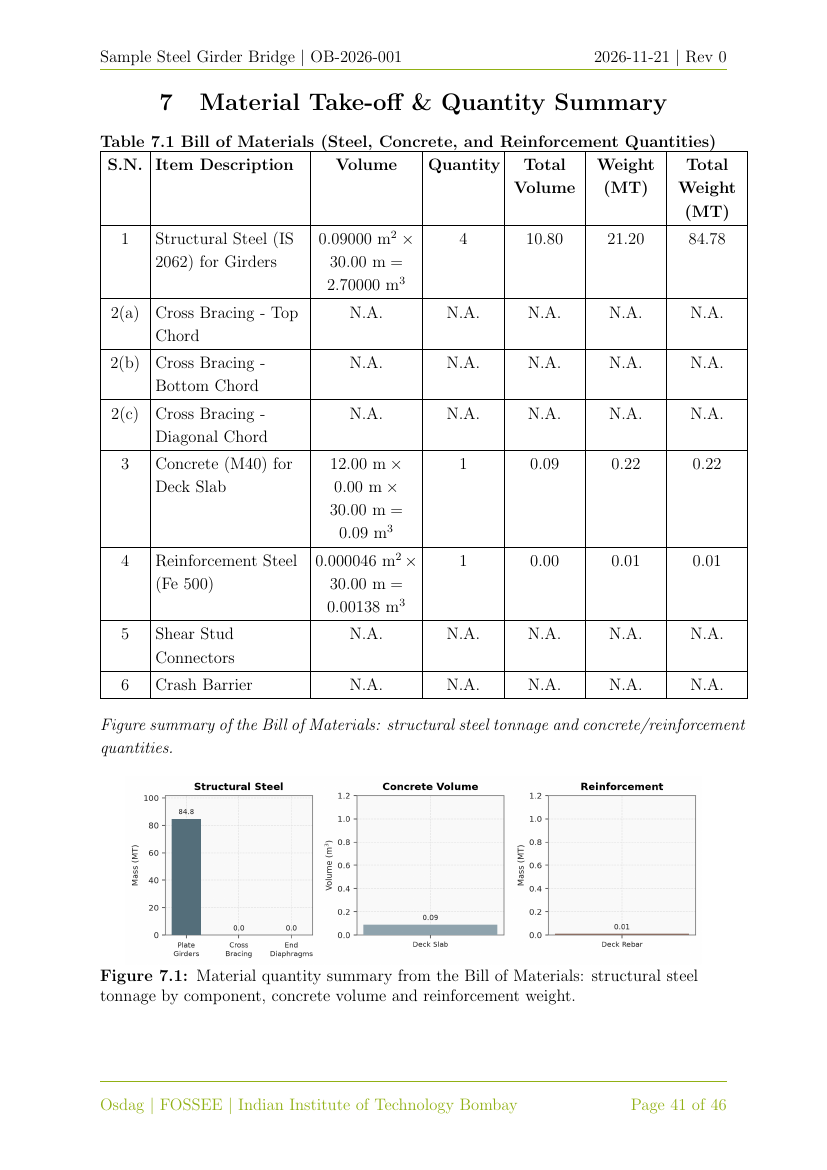
\includegraphics[width=0.78\linewidth]{report_assets/material_chart}
\caption{Material quantity chart (Chapter 7).}
\end{figure}
\begin{figure}[htbp]
\centering
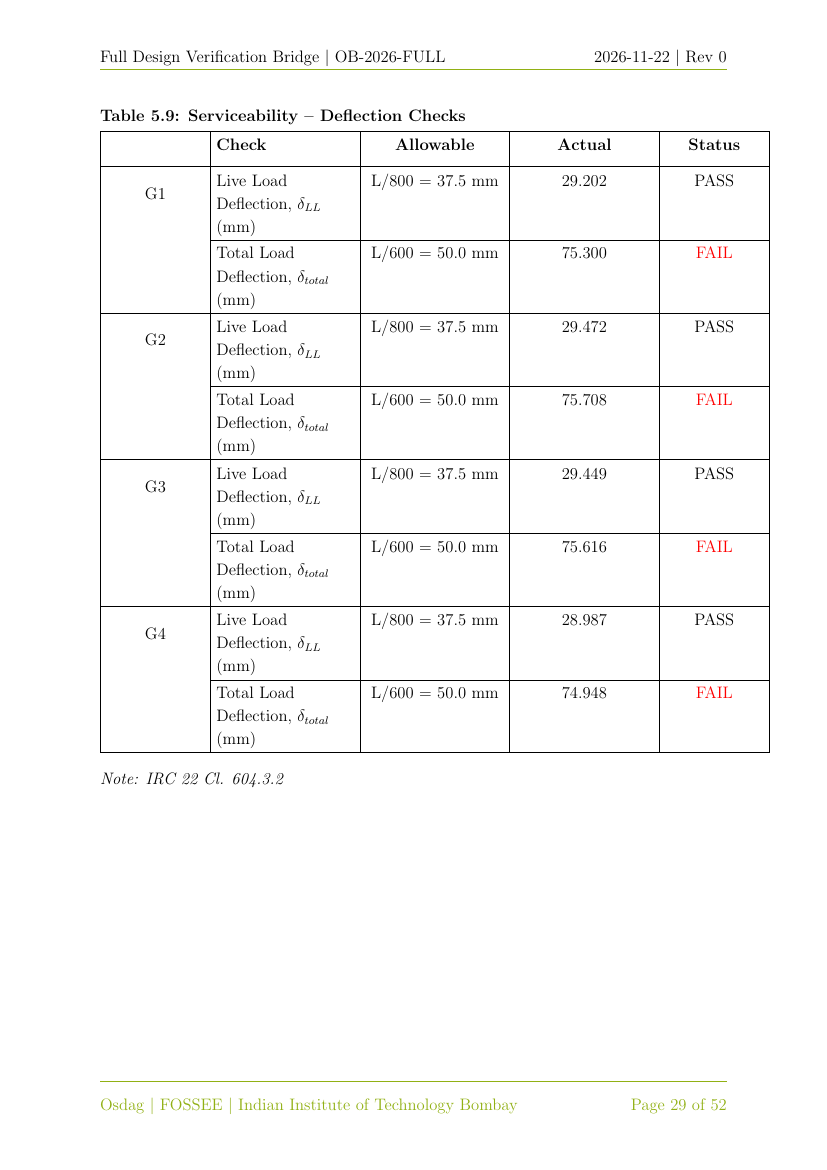
\includegraphics[width=0.78\linewidth]{report_assets/real_page30}
\caption{Real-design report, Page 30: G4 rows clear of footer, header repeated.}
\end{figure}

\section{Reproduction}
\begin{verbatim}
PYTHONPATH=src python -m pytest tests/unit/test_report_styles.py -q
python scripts/generate_sample_reports.py deliverables Report_After
QT_QPA_PLATFORM=offscreen PYTHONPATH=src python scripts/gui_smoke_test.py
PYTHONPATH=src python scripts/run_full_design_test.py
\end{verbatim}

\section{Scope review: remaining internship tasks}
With the environment now available (PySide6, OpenSeesPy, ifcopenshell installed):
\begin{itemize}
\item \textbf{Osdag UI / 2D CAD / plotting} --- feasible next; PySide6 and OpenSees are present.
\item \textbf{Osdag 3D substructure + IFC} --- blocked on \texttt{pythonocc-core}, which is conda-only and unavailable here.
\item \textbf{eSim tasks} --- require eSim / KiCad installations not present in this environment.
\end{itemize}

\end{document}
